\documentclass{beamer}
\usetheme{Goettingen}
\usecolortheme{crane}

% balíčky

\usepackage[utf8]{inputenc}
\usepackage[czech]{babel}
\usepackage{graphicx}

% informace o dokumentu

\title[Slackline]
{Slackline - nejenom zábava}
\subtitle{Novodobý sport, který baví i léčí}
\author{Matěj Mitaš}
\date{\today} % (optional)

% text dokumentu

\begin{document}

% titulní stránka
% (název prezentace, autor, datum...)

\begin{frame}
  \titlepage
\end{frame}

% obsah prezentace
% (používají se klasické sekce)

\section{Úvod}

\begin{frame}
  \frametitle{Slackline}
  \framesubtitle{O co se tedy jedná?}
  
  \begin{itemize}
		\item Slackline vznikla z anglického slova \uv{slack}, v překladu znamenající \uv{volný, rozevlátý}.
		\item Tento sport definován chůzí, balancováním a skoky na různě napnutém popruhu.
		\item Pracuje se buď s $2.5cm$ nebo $5cm$ širokým popruhem.
		\item Existuje více poddisciplín, budou probrány na dalších slidech.
		\item V České Republice se tento sport těší značné oblibě.
	\end{itemize}
\end{frame}

\section{Časová osa}

\begin{frame}
  \frametitle{Vznik}
  % ...
  
    \begin{itemize}
		\item Počátky tohoto sportu se datují do 70.let minulého století.
		\item První experimentátoři se vynořili v parku Yosemite v USA.
		\item Slackline vzešla z lezecké komunity, je s ní nadále pevně svázaná.
		\item Z tohoto důvodu se za královskou disciplínu považuje \uv{highline}.
	\end{itemize}
\end{frame}

\begin{frame}
  \frametitle{Ranná léta a slackline v ČR}
  
  \begin{itemize}
		\item Vše začalo v 70.letech, ale trvalo další dvě dekády, než se tento sport dostal do hledáčku světové veřejnosti.
		\item Po přelomu milénia se začalo debatovat o profesionalizaci, avšak z těchto úvah až donedávna sešlo
		\item Kolem roku 2007 došlo k profesionalizaci, stejně tak jako k založení světové asociace.
		\item O slackline se v České Republice dlouho vědelo z doslechu, avšak po roce 2010 se situace notně zlepšila.
	\end{itemize}
  % ...
\end{frame}

\section{Disciplíny}

\begin{frame}
  \frametitle{Disciplíny}
  
  \begin{itemize}
		\item Jak bylo výše zmíněno, slackline se dělí na více disciplín.
		\item Nejběžnější je \uv{longline}, cílem je přejít co nejdelší vzdálenost (aktuální rekord $806m$)
		\item Divácky nejpopulárnější je zajisté \uv{trickline}, která ve zkratce řečeno gymnastika.
		\item Královskou disciplínou je \uv{highline}, která se provozuje ve značných výškách (od $20m$ výše, aktuální rekord $1023m$).
  \end{itemize}
  % ...
\end{frame}

\begin{frame}
  \frametitle{Longline}
  
  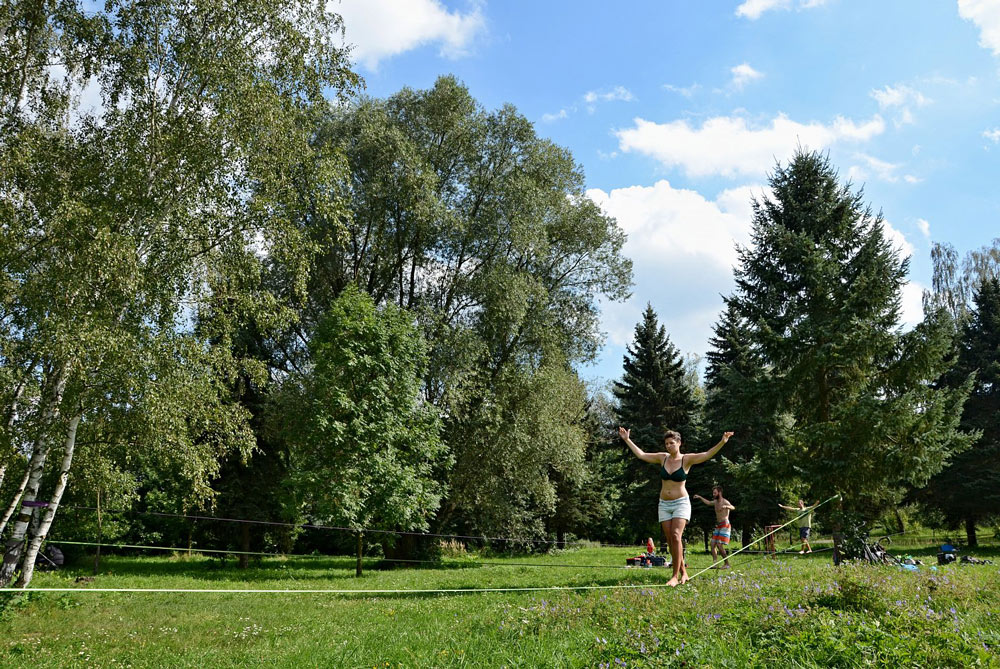
\includegraphics[width=275pt]{longline.jpg}
  % ...
\end{frame}

\begin{frame}
  \frametitle{Trickline}
  
  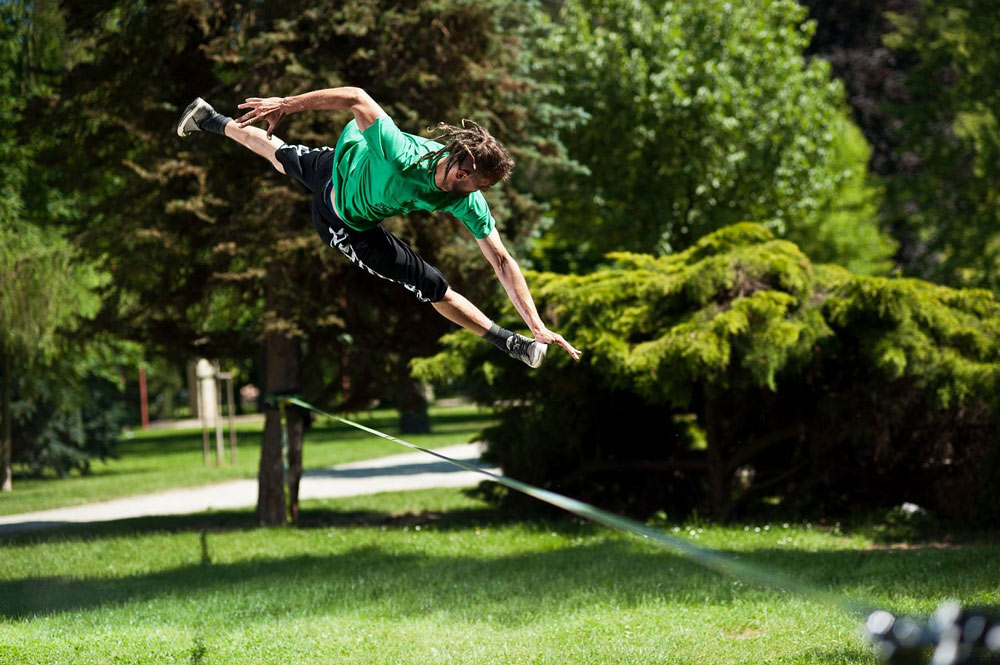
\includegraphics[width=275pt]{trickline.jpg}
  % ...
\end{frame}

\begin{frame}
  \frametitle{Highline}
  
  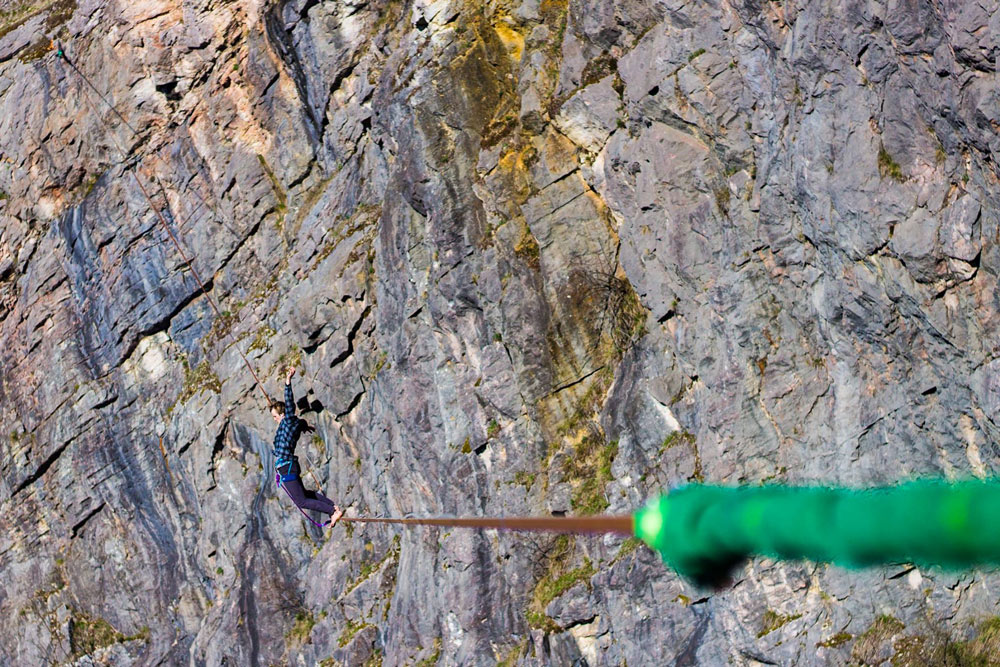
\includegraphics[width=275pt]{highline.jpg}
  % ...
\end{frame}

\section{Zdroje}

\begin{frame}
  \frametitle{Použité zdroje}
  
  \begin{itemize}
		\item archiv autora
		\item web www.slackline.cz
	\end{itemize}
  % ...
\end{frame}

\end{document}